%------------------------------%
%% ✎ Dylan (V1) %%%%%%%%% ✅ %%
%% ✎ Alain (V2) %%%%%%%%% ❌ %%
%% ✎ Dylan (V3) %%%%%%%%% ❌ %%
%------------------------------%

\afterpage{%
\afterpage{%

    % Arrière-plan partie II
    \AddToShipoutPictureBG*{%
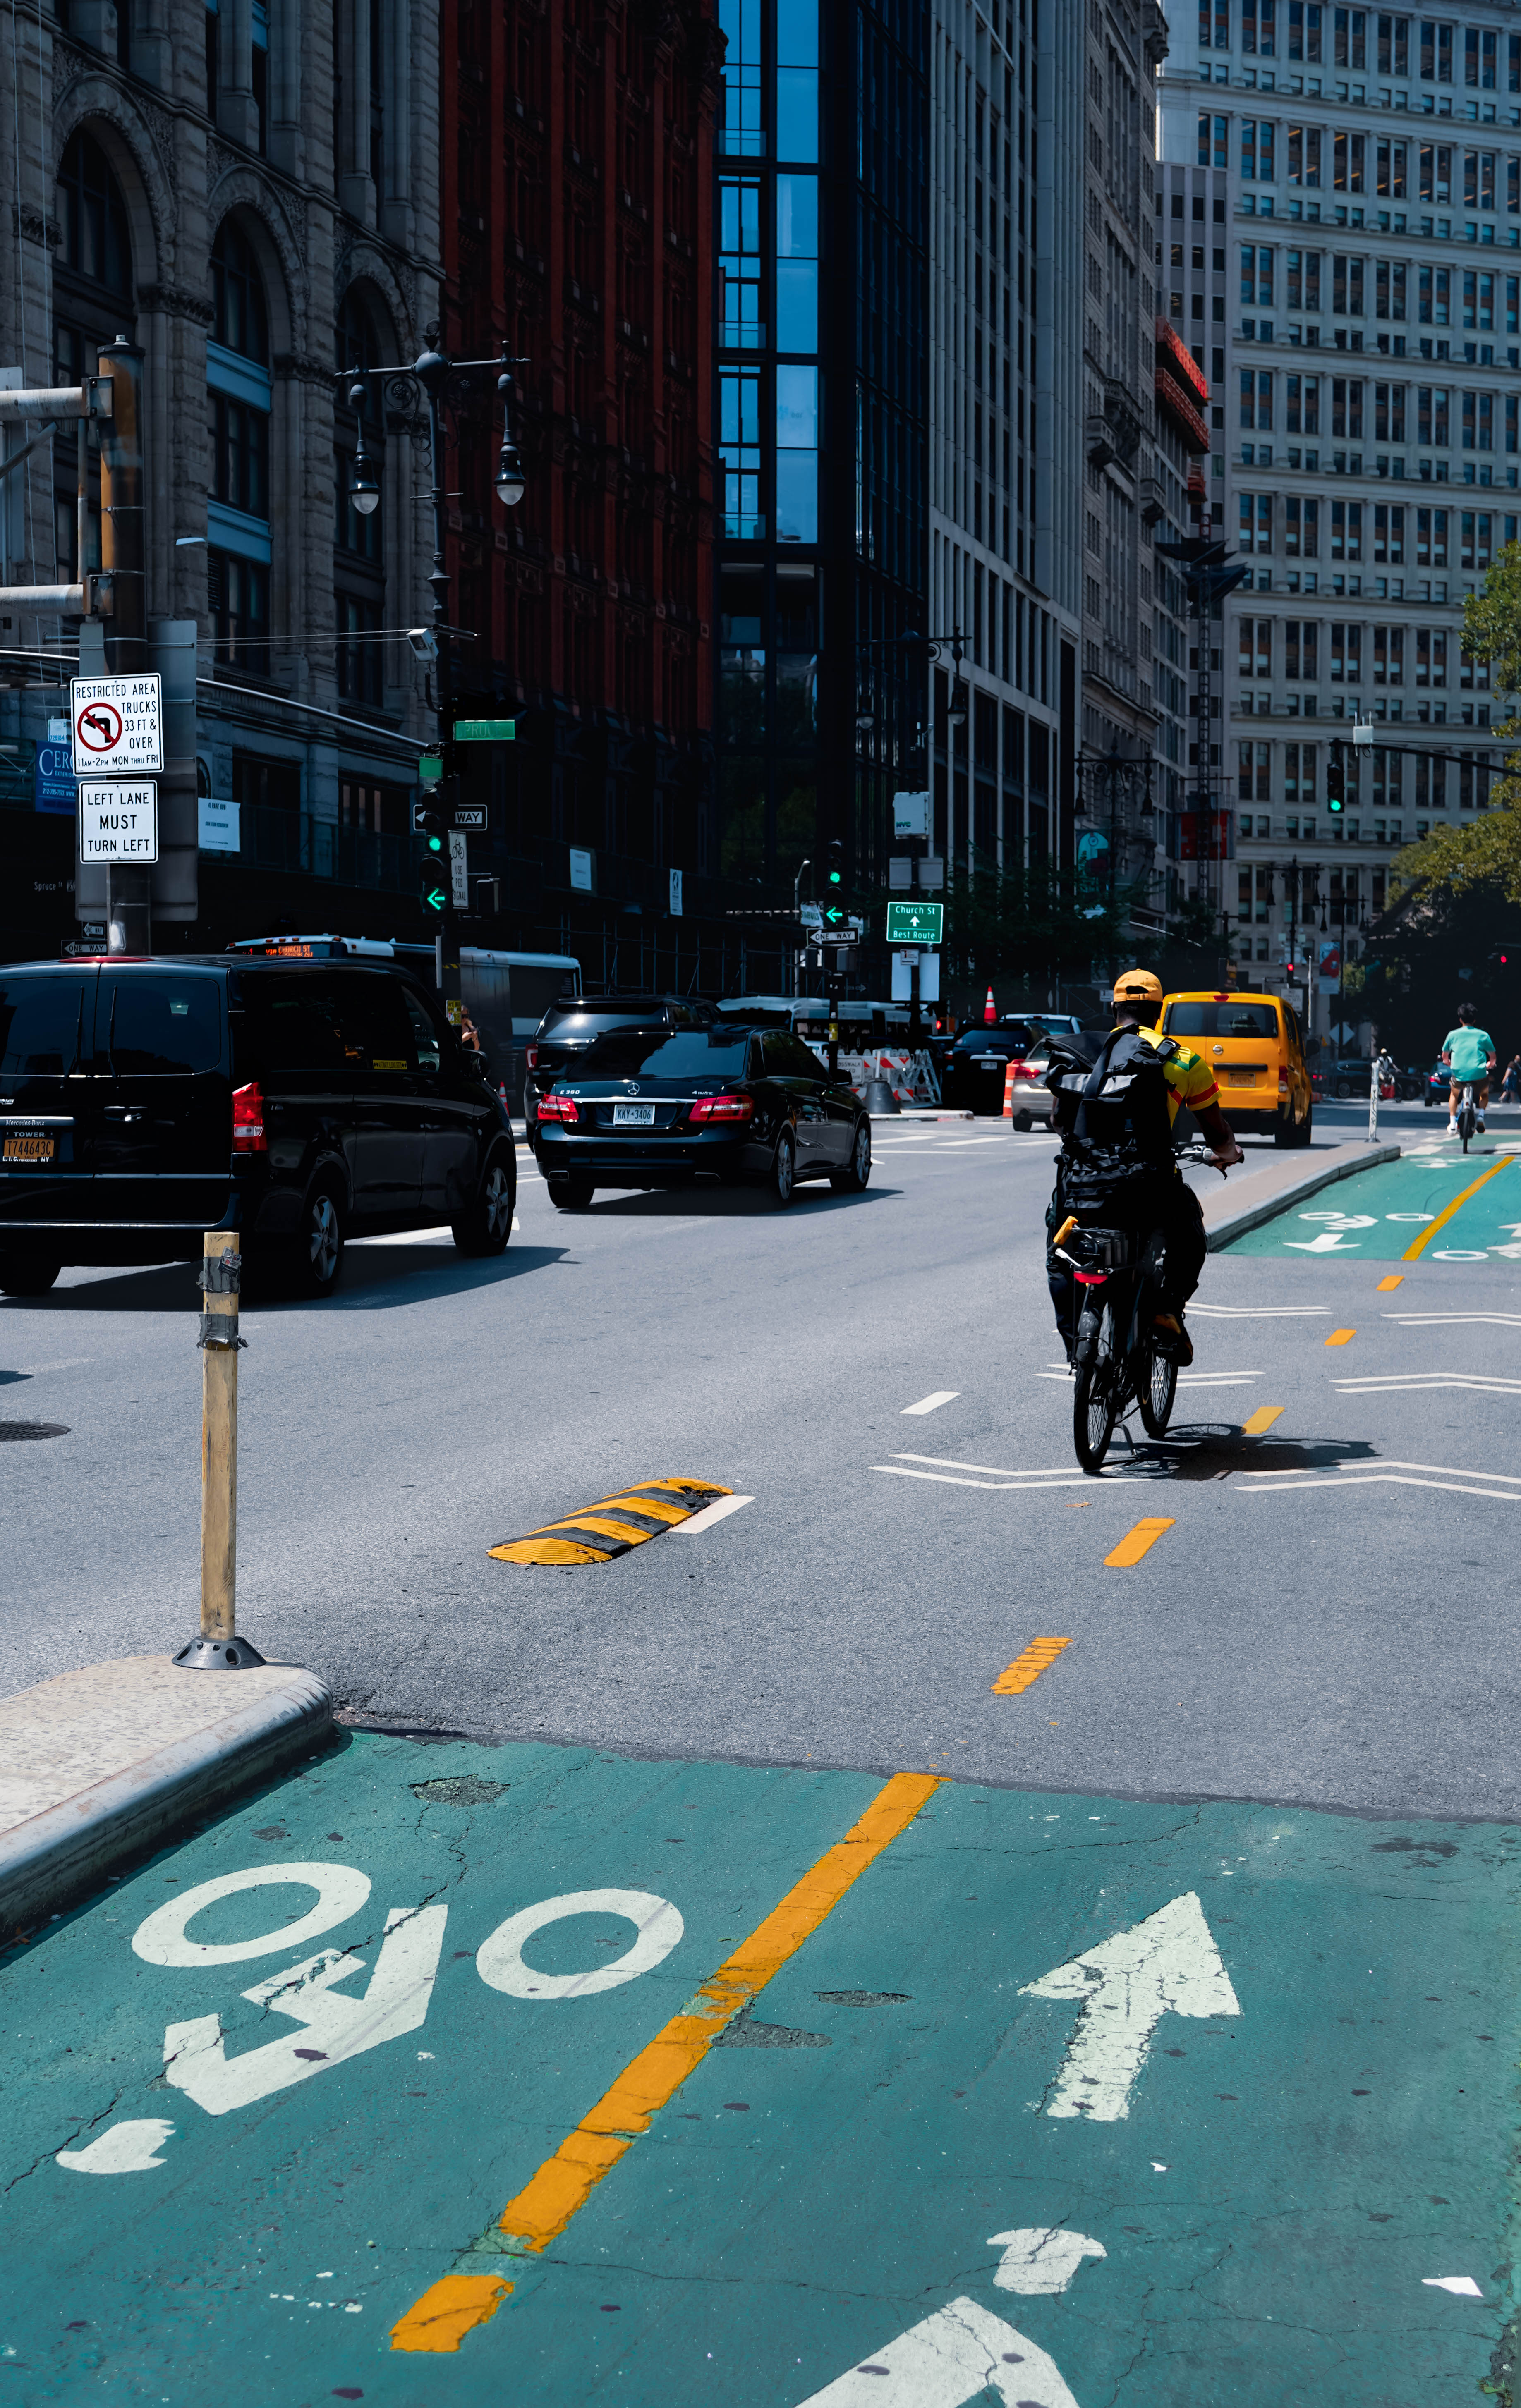
\includegraphics[width=\paperwidth,height=\paperheight]{src/Figures/Arriere_plan/Arriere_plan_Part_2.jpg}
    }

% Rectangle
\AddToShipoutPictureBG*{
  \begin{tikzpicture}[remember picture,overlay]
    \node[fill=white, opacity=0.75, text width=\paperwidth, minimum height=10cm, anchor=north] 
    at ([yshift=-7.7cm]current page.north) {};
  \end{tikzpicture}
}

% Source
\AddToShipoutPictureFG*{
  \AtPageLowerRight{
    \raisebox{1cm}{
      \hspace{16cm}
      
\begin{tikzpicture}
        \node[fill=white, rounded corners=5pt, inner sep=5pt, align=center] {
          \tiny{Photographie~: \textcolor{blue}{Dylan Moinse (2023)}}
        };
      \end{tikzpicture}
    }
  }
}
}}

\needspace{1\baselineskip} % Réserve de l'espace
\part{Le potentiel d’extension et de transformation des quartiers de gare par l'usage intermodal de la mobilité individuelle légère
    \label{part2:titre}
    }
    \markboth{Partie~II~: Pratiques intermodales et gains d'accessibilité}{}
    \markright{Partie~II~: Pratiques intermodales et gains d'accessibilité}{}

% Introduction de la partie II
\cleardoublepage
\section*{Introduction de la partie~II
    \label{part2:introduction}
    }
    \addcontentsline{toc}{chapter}{Introduction de la partie~II}

    % Introduction
\lettrine[lines=3, findent=8pt, nindent=0pt]{\lettrinefont C}{ette} deuxième partie a pour objectif de documenter et d'analyser les usages de la mobilité individuelle légère en complémentarité avec le transport public, et d'évaluer son impact sur l'organisation spatiale des quartiers de gare. Elle s'attache ainsi à étudier les dynamiques d'usage, en identifiant les facteurs influençant les choix modaux qui s'opèrent, ainsi que les effets spatiaux et territoriaux de la mobilité individuelle légère sur les espaces ferroviaires et leur périmètre fonctionnel. En s'interrogeant sur les interactions entre infrastructure, pratiques de mobilité et structuration urbaine, cette partie vise à éclairer le rôle stratégique de la mobilité individuelle légère dans l'évolution des quartiers de gare, en lien avec la notion d'accessibilité.%%Rédigé%%

    % Chapitre 4
\textsl{Rendre compte des pratiques de mobilité et du profil des cyclo-voyageur·se·s ayant recours à la mobilité individuelle légère} (\hyperref[objectif-4]{objectif~\(O_4\)}, page~\pageref{objectif-4}). \hyperref[chap4:titre]{Le quatrième chapitre} (page~\pageref{chap4:titre}) se consacre à étudier l'usage et la pratique intermodale associant transport public et mobilité individuelle légère. Il aborde la question légitime de la proportion d'usager·ère·s combinant ces modes de déplacement en tirant parti de l'exploitation des données d'observation quantitative, de sorte à objectiver la place de la mobilité individuelle légère au sein de la chaîne de déplacement intermodale. Cette étude est complétée par l'analyse du questionnaire qui permet de mieux cerner le profil socio-démographique de ces groupes sociaux, ainsi que les facteurs influençant leurs choix modaux et, par conséquent, les principaux freins à l'adoption de ces formes de mobilité. L'approche qualitative basée sur les entretiens mobiles permet, en révélant des éléments souvent invisibles dans les données quantitatives, de discuter de l'expérience et de la perception des usager·ère·s, en soulevant les stratégies de mobilités mises en place et en permettant de comprendre les arbitrages modaux et les motivations. En croisant ces niveaux d'analyse, ce chapitre dresse un portrait détaillé et original des utilisateur·rice·s et de leurs pratiques de mobilité, du fait de la précision des informations recueillies, qui permettent de mettre en perspective les diverses formes de combinaison modale existantes.%%Rédigé%%

    % Chapitre 5
\textsl{Décrypter les implications spatiales de la mobilité individuelle légère en matière d'accessibilité intermodale} (\hyperref[objectif-5]{objectif~\(O_5\)}, page~\pageref{objectif-5}). \hyperref[chap5:titre]{Le cinquième chapitre} (page~\pageref{chap5:titre}) interroge, au-delà des pratiques de mobilité individuelles, les effets territoriaux de l'essor de l'usage, potentiel comme effectif, de la mobilité individuelle légère s'inscrivant dans les quartiers de gare. Il s'agit d'évaluer dans quelle mesure ce rapport à la proximité transforme l'organisation des espaces ferroviaire et élargit l'accessibilité aux gares. Ce chapitre mobilise une analyse spatiale permettant de mesurer les gains d'accessibilité générés par l'intégration de la mobilité individuelle légère. L'accessibilité inter-nodale et intermodale a ainsi été modélisée afin de comparer les périmètres fonctionnels des quartiers de gare selon la portée de chaque mode de déplacement. Cette démarche vient redéfinir les distances acceptables et ainsi déterminer le potentiel d'extension de la zone d'influence des transports en commun, à l'échelle locale, et l'amélioration de la desserte ferroviaire, dans le périmètre régional. En complément, nous nous sommes intéressés aux choix d'itinéraire des cyclo-voyageur·se·s afin d'identifier les parcours privilégiés, en fonction de la présence d'infrastructure et de types d'aménagement urbain. Ce regard géographique permet d'appréhender les logiques d'appropriation de l'espace par les individus mobiles et de nous intéresser à la compatibilité des aménagements actuels avec les besoins exprimés.%%Rédigé%%